% !TEX program = xelatex
% !TEX root = 05_abbildungen_tikz.tex
% !TEX encoding = UTF-8 Unicode
% !TEX spellcheck = de_DE
% 
% © 2016 Moritz Brinkmann, CC-by-sa
% http://latexkurs.github.io

Der Baum in Abbildung \ref{fig:tree} wurde mit folgendem Code erstellt:
\begin{lstlisting}
\usetikzlibrary{trees}

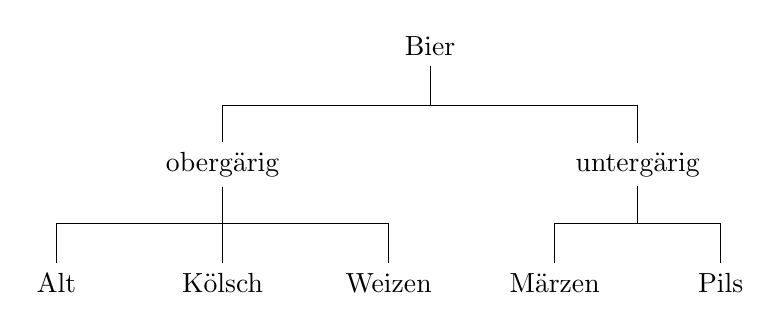
\begin{tikzpicture}[
  edge from parent fork down,
  level 1/.style={sibling distance=15em},
  level 2/.style={sibling distance=6em},
]
  \node {Bier}
    child {node {obergärig}
      child {node {Alt}}
      child {node {Kölsch}}
      child {node {Weizen}}
    }
    child {node {untergärig}
      child {node {Märzen}}
      child {node {Pils}}
    }
  ;
\end{tikzpicture}
\end{lstlisting}